\subsubsection{数据结构概览}

所谓数据结构，就是指数据的组织、存储、操作和处理方式。数据结构是计算机科学中最基本的概念之一，
是计算机程序设计的基础。基本的操作有四：\textbf{插入、删除、改动、查找}（增删改查）。

下面我们将简单介绍几种常见的数据结构，以及它们的STL容器：

\begin{enumerate}
    \item \textbf{数组（Array）}：相同类型的元素按顺序存储在一块连续内存中的线性结构，
    可以通过下标在 $O(1)$ 时间内直接访问任意元素。
    \item \textbf{链表（Linked List）}：由一系列在内存中不连续的节点串成的线性结构，
    每个节点存储数据和指向下一个节点的指针；已知位置时插入、删除只需改变指针，
    但查找必须从头节点开始逐个遍历。
    \item \textbf{队列（Queue）}：先进先出（FIFO，First In First Out）的线性结构，
    只允许在队尾插入元素、在队头删除元素，先进入的元素先被取出。
    \item \textbf{优先队列（Priority Queue）}：每个元素都带有一个优先级的队列，
    每次出队的不是最早进入的元素，而是当前优先级最高的元素。
    \item \textbf{堆栈（Stack）}：后进先出（LIFO，Last In First Out）的线性结构，
    插入（压栈）和删除（弹栈）都只能在栈顶一端进行。
    \item \textbf{树（Tree）}：一种非线性结构，其中有且仅有一个根节点，
    其余每个节点都恰好有一个父节点；任意两个节点之间有且仅有一条路径相连，即树中不存在环路。
    \item \textbf{二叉树（Binary Tree）}：每个节点至多有两个子节点的树，
    两个子节点区分左右，分别称为左子节点和右子节点。
    \item \textbf{堆（Heap）}：满足"堆性质"的完全二叉树——最大堆中每个节点的值都大于或等于其子节点，
    最小堆则相反；因此堆顶永远是最大值（或最小值）。
\end{enumerate}

它们的头文件如下：

\begin{tcode}
#include <array>    //静态数组array
#include <vector>   //动态数组vector
#include <list>     //链表list
#include <queue>    //队列queue 优先队列priority_queue
#include <stack>    //堆栈stack
#include <map>      //映射map 是一种快速查找关联容器
\end{tcode}

需要注意的是，上面所列举的数据结构类型并不是并列的，三大数据结构分别是：线性表（包括1、2、3、4、5）
，树（包括6、7、8），图（太复杂，暂时不介绍）。

\subsubsection{顺序容器}
\textbf{数组与 vector。}

数组是最基本的数据结构，它是一组相同类型的数据，按照顺序存储在一块连续的内存中，如图\ref{fig:数组}。

\begin{figure}[H]
    \centering
    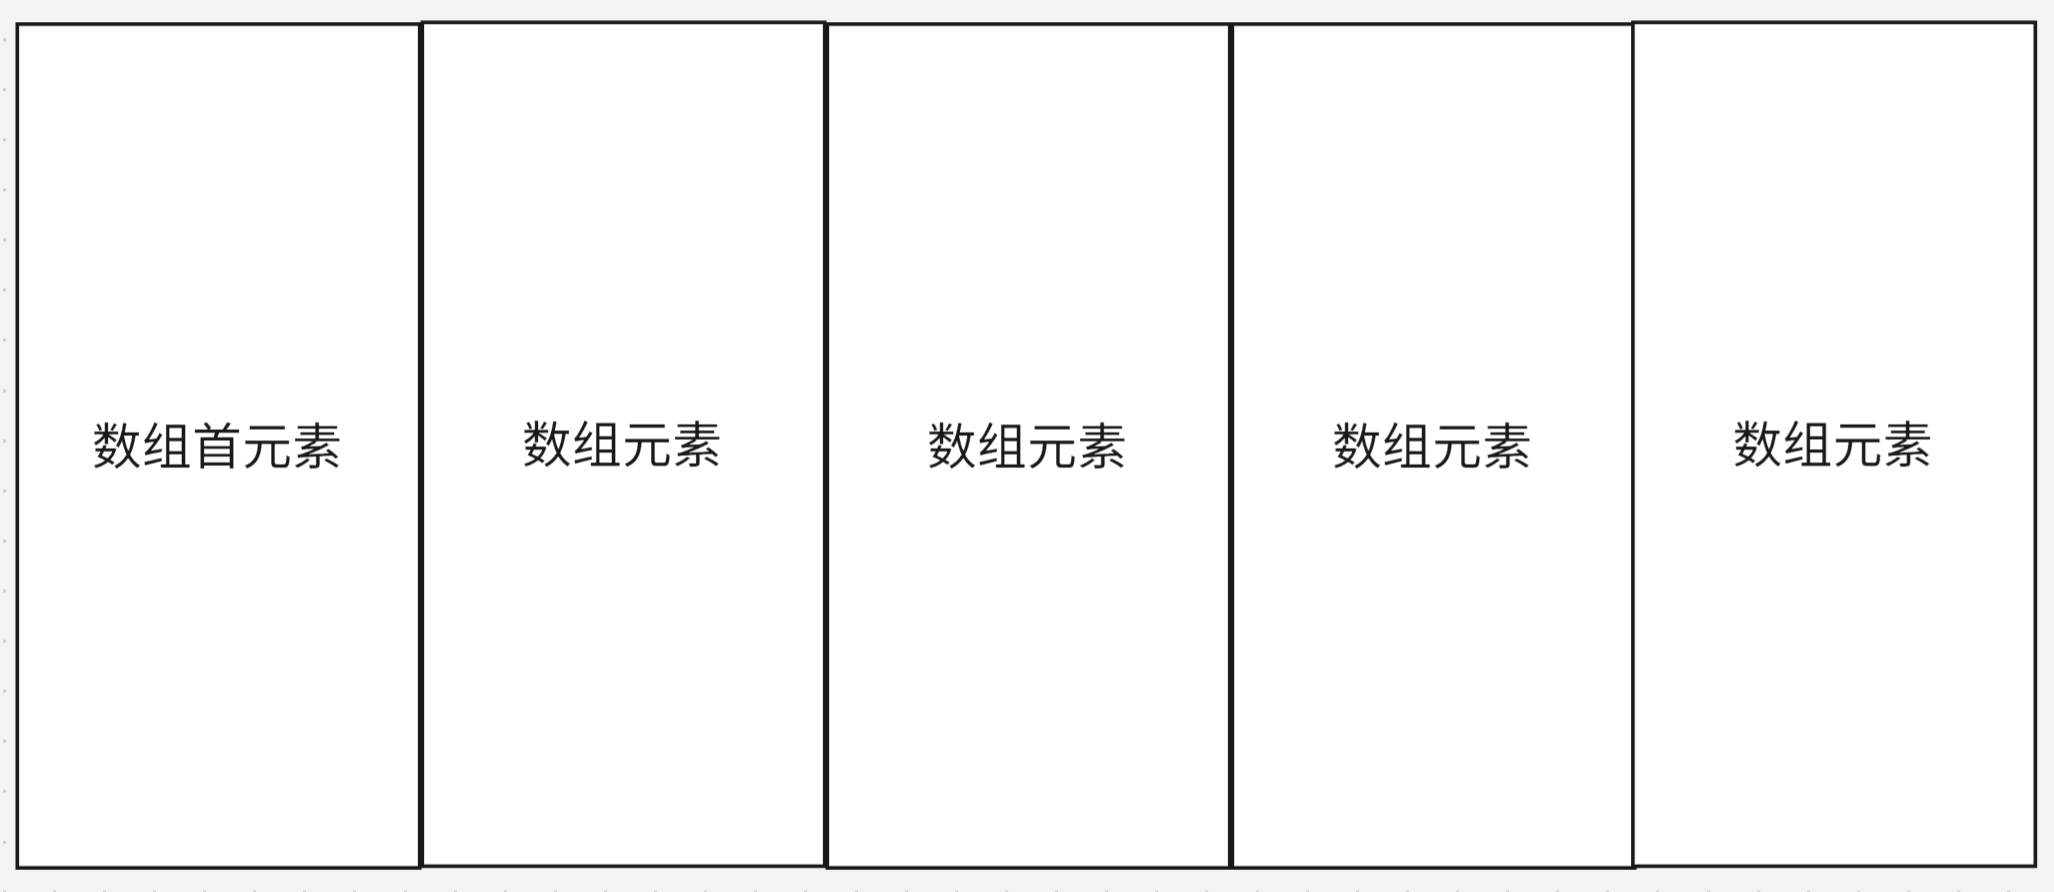
\includegraphics[width=0.7\textwidth]{数组.png}
    \caption{数组} % 图片标题
    \label{fig:数组} % 图片标签，用于引用
\end{figure}

\textbf{数组（Array）}，又称\textbf{顺序表}，它的STL容器有两种，分别是$array$和$vector$。

$array$是固定大小的数组。$vector$是一种动态数组，可以动态增长，可以根据需要自动分配内存。两者的声明方式如下：
\begin{tcode}
std::array<int,5> arr;
std::vector<int> vec;
\end{tcode}

$array$并不常用，因为它是固定大小的，如果需要改变大小，只能重新声明一个新的数组。

\begin{note}
想详细了解 \texttt{array} 可以参考这篇 blog：

\url{https://blog.csdn.net/qq_38410730/article/details/102802239}
\end{note}

$vector$由于其动态性，可以根据需要自动分配内存，因此使用起来比较方便，在工程实践中也更常用。
$vector$的实现原理是当检测到$vector$的容量不足时，会自动分配新的内存（原来的大小$\times$2），并将原有数据复制到新内存中。
这个复制的过程非常缓慢，因此，在使用大型的资源时，$vector$的效率可能会比较低。

\begin{example}
\texttt{vector} 的常用成员函数：
\begin{tcode}
#include <vector>

std::vector<int> vec{1,2,3,4,5,6};
vec[0];         //访问（快速）
vec.at(0);      //访问（安全，越界会抛异常）
vec.front();    //第一个元素
vec.back();     //最后一个元素
vec.empty();    //检查是否为空
vec.size();     //返回容器大小
vec.reserve(10);//预留空间，避免反复扩容
vec.clear();    //清除所有元素
vec.insert(vec.begin(),1);//插入元素
vec.erase(vec.begin());//删除元素
vec.push_back(1); //在最后添加
vec.emplace_back(); //在最后原位构造，省去一次拷贝
vec.pop_back();     //删除最后一个
\end{tcode}
\end{example}

\textbf{链表。}

链表是一种非连续的内存块，它是由一系列节点组成，每个节点都包含数据和指针。
链表的实现原理是每个节点都包含一个指针，指向下一个节点。链表的头节点称为头指针，尾节点称为尾指针。
链表的插入、删除操作都比较容易，只需要改变指针即可，但是查找操作比较麻烦，需要从头节点开始遍历。

\begin{note}
理论上链表的插入删除是 $O(1)$、数组的中间插入是 $O(n)$，但实际工程中链表经常\textbf{跑不过} vector：
链表的节点分散在内存各处，CPU 缓存（Cache）帮不上忙，每次访问都可能发生缓存未命中；
而 vector 的内存是连续的，缓存预取非常友好。所以除非有频繁的中部插入删除，否则默认选 vector。
\end{note}
\begin{figure}[H]
    \centering
    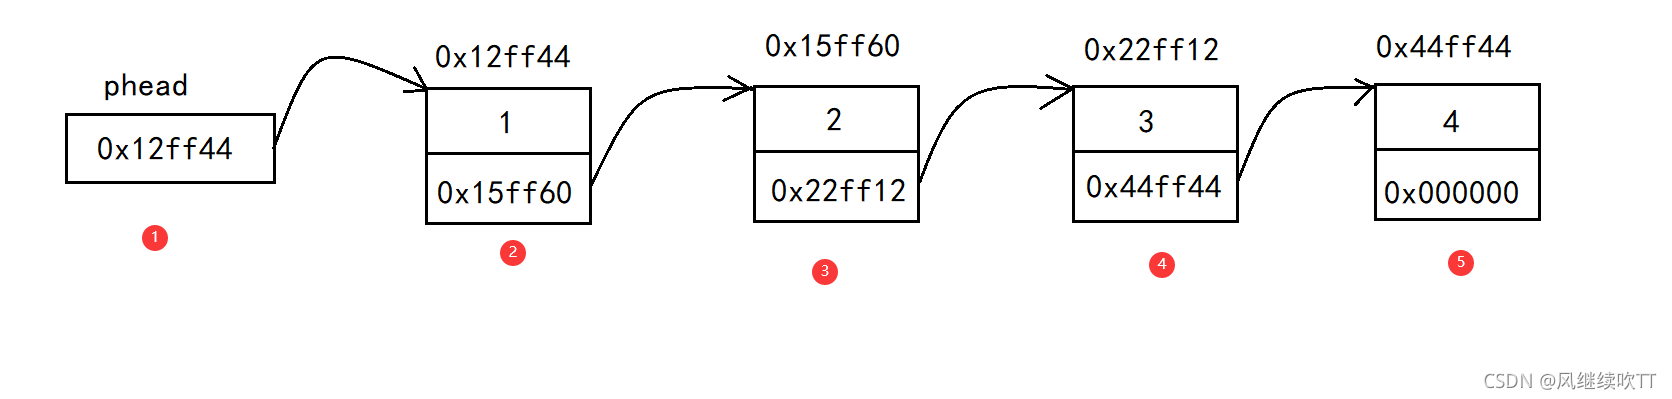
\includegraphics[width=0.7\textwidth]{链表1.png}
    \caption{链表} % 图片标题
    \label{fig:链表} % 图片标签，用于引用
\end{figure}

它的STL容器是$list$（双向链表）和$forward\_list$（单向链表）。比较简单，请自行查阅相关文档：

\url{https://zh.cppreference.com/w/cpp/container/list}

\begin{exercise}
向 \texttt{std::vector<int>} 中依次 \texttt{push\_back} 数字 $1 \sim 10$，在每次插入后打印 \texttt{size()} 和 \texttt{capacity()}，
观察容量翻倍的时机，验证"容量不足时扩容为原来 2 倍"的说法。
\end{exercise}

\subsubsection{队列、优先队列与堆栈}
\textbf{队列。}

队列是一种线性数据结构，它按照\textbf{先进先出}的原则进行操作。队列有两个基本操作，分别是\textbf{入队}和\textbf{出队}。入队操作是在队列的末尾添加一个元素，而出队操作是从队列的头部移除一个元素。队列有两个端点，队头和队尾，队头是队列的第一个元素，出队操作发生的地方，队尾是队列的最后一个元素，入队操作发生的地方。通常情况下，\textbf{不允许随机访问}队列中的元素，只能访问队头元素。
队列在\textbf{多任务处理、打印任务管理、缓冲处理}等场景中有广泛应用，它帮助维持操作的顺序和流程控制。
（很常用）
\begin{figure}[H]
    \centering
    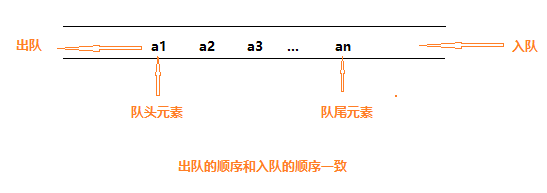
\includegraphics[width=0.7\textwidth]{队列1.png}
    \caption{入队和出队操作} % 图片标题
    \label{fig:入队和出队操作} % 图片标签，用于引用
\end{figure}
\begin{figure}[H]
    \centering
    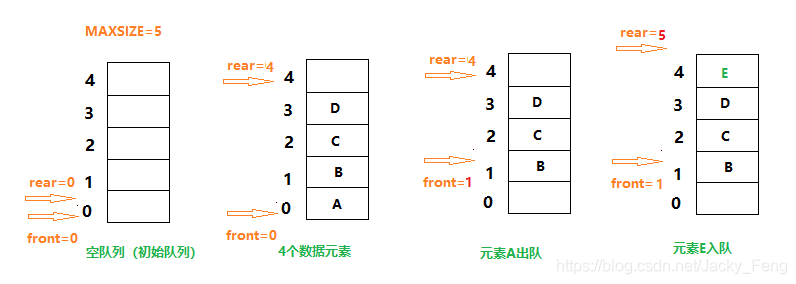
\includegraphics[width=0.7\textwidth]{队列2.png}
    \caption{队列实现方式} % 图片标题
    \label{fig:队列实现方式} % 图片标签，用于引用
\end{figure}

它的STL容器是$deque$，基于双向队列，C++还实现了3种容器适配器：
$stack$（堆栈）、$queue$（单向队列）、$priority\_queue$（优先队列）。相较于$deque$，我们更常用$queue$
进行队列操作。

\begin{note}
具体用法请自行查阅相关文档：

\url{https://zh.cppreference.com/w/cpp/container/deque}

\url{https://zh.cppreference.com/w/cpp/container/queue}
\end{note}

\textbf{优先队列。}

优先队列是一种特殊的队列，它允许插队的出现，可以根据“重要性”对队中元素进行排序。
优先队列的实现原理是每个元素都有一个优先级，优先级越高，元素越容易被取出。
优先队列的应用场景有很多，如任务调度、排序、搜索等。

\begin{figure}[H]
    \centering
    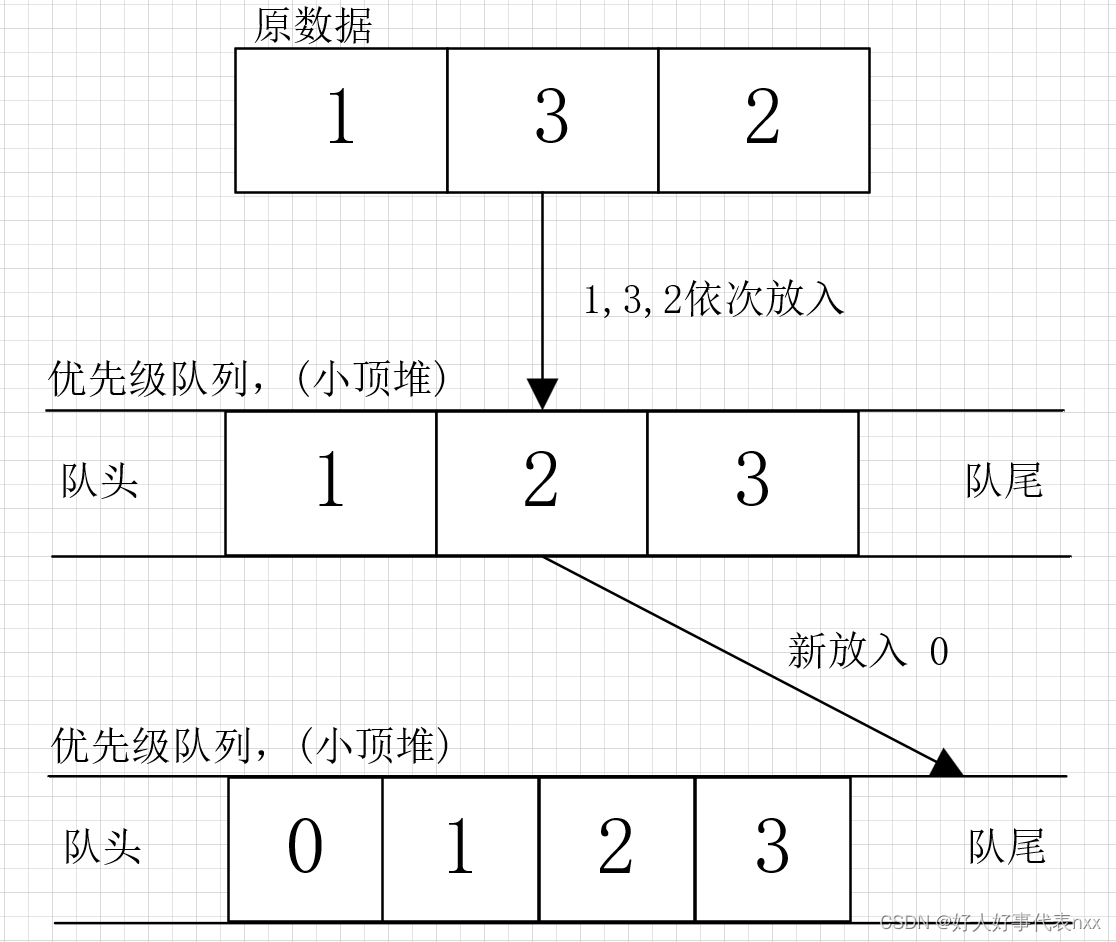
\includegraphics[width=0.7\textwidth]{优先队列1.png}
    \caption{优先队列} % 图片标题
    \label{fig:优先队列} % 图片标签，用于引用
\end{figure}

它的实现是容器适配器$priority\_queue$，
具体用法请自行查阅相关文档：

\url{https://zh.cppreference.com/w/cpp/container/priority_queue}

\textbf{堆栈。}

堆栈是一种线性数据结构，它按照\textbf{先进后出}的原则进行操作。堆栈有两个基本操作，分别是\textbf{压栈}和\textbf{弹栈}。压栈操作是在堆栈的顶部添加一个元素，而弹栈操作是从堆栈的顶部移除一个元素。堆栈有两个端点，栈顶和栈底，栈顶是堆栈的顶部，压栈操作发生的地方，栈底是堆栈的底部，弹栈操作发生的地方。
堆栈在\textbf{函数调用、表达式求值、回溯、计算器、括号匹配、迷宫寻路}等场景中有广泛应用。

\begin{figure}[H]
    \centering
    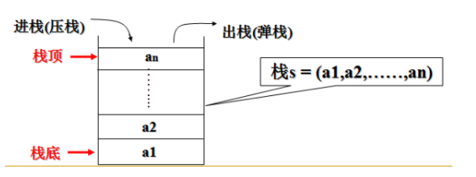
\includegraphics[width=0.7\textwidth]{堆栈1.png}
    \caption{压栈和弹栈操作} % 图片标题
    \label{fig:压栈和弹栈操作} % 图片标签，用于引用
\end{figure}
\begin{figure}[H]
    \centering
    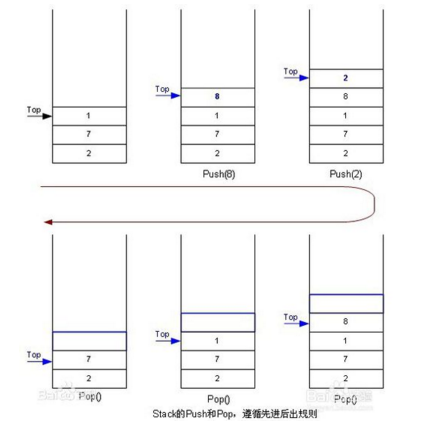
\includegraphics[width=0.7\textwidth]{堆栈2.png}
    \caption{堆栈实现方式} % 图片标题
    \label{fig:堆栈实现方式} % 图片标签，用于引用
\end{figure}

它的实现是容器适配器$stack$，
具体用法请自行查阅相关文档：

\url{https://zh.cppreference.com/w/cpp/container/stack}

\begin{exercise}
使用 \texttt{std::stack<char>} 编写括号匹配检查：读入一串只含 \texttt{(}、\texttt{)} 的字符串，
判断括号是否配对（提示：遇左括号压栈，遇右括号弹栈，弹空或结束时栈非空则不匹配）。
\end{exercise}

\subsubsection{树与堆}
\textbf{树。}

树是一种非线性数据结构，由若干\textbf{节点（Node）}和连接节点的\textbf{边（Edge）}组成。
它有且仅有一个根节点（Root），其余每个节点都恰好有一个父节点，从根节点出发可以到达任意节点，
且任意两个节点之间有且仅有一条路径——也就是说，树里不存在环路。

树还有一个更本质的\textbf{递归定义}：一棵树要么是空树；要么由一个根节点和若干棵互不相交的子树组成，
而每棵子树本身也是一棵树。"树的每个部分还是树"——正是这种自相似的结构，
让递归成为处理树最自然的方式（遍历、求高度、搜索都一行递归搞定）。

树的种类很多，如二叉树、二叉搜索树、AVL树、红黑树、B树、B+树、B*树等。
\begin{figure}[H]
    \centering
    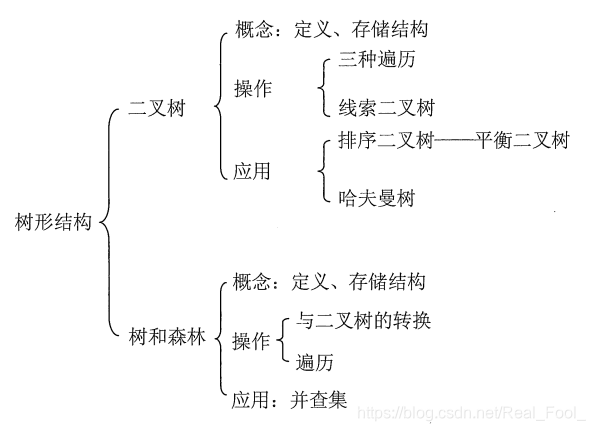
\includegraphics[width=0.7\textwidth]{树1.png}
    \caption{树的逻辑图（了解即可）} % 图片标题
    \label{fig:树的逻辑图} % 图片标签，用于引用
\end{figure}

\begin{figure}[H]
    \centering
    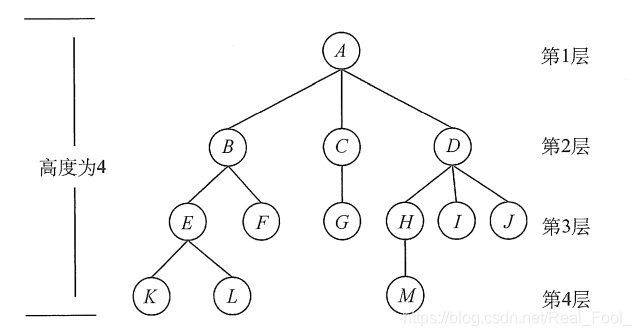
\includegraphics[width=0.7\textwidth]{树2.png}
    \caption{树的示意图} % 图片标题
    \label{fig:树的示意图} % 图片标签，用于引用
\end{figure}

\textbf{堆。}

堆是一种特殊的树，它是一个\textbf{完全二叉树}，即除叶节点外，其他的每个节点都有两个子节点。
每个节点都有一个值，并且每个节点\textbf{都大于或等于其子节点}（这是最大堆max-heap，类似的，还有最小堆min-heap）。堆的应用场景有很多，如排序、优先队列、图算法、堆排序等。

\begin{figure}[H]
    \centering
    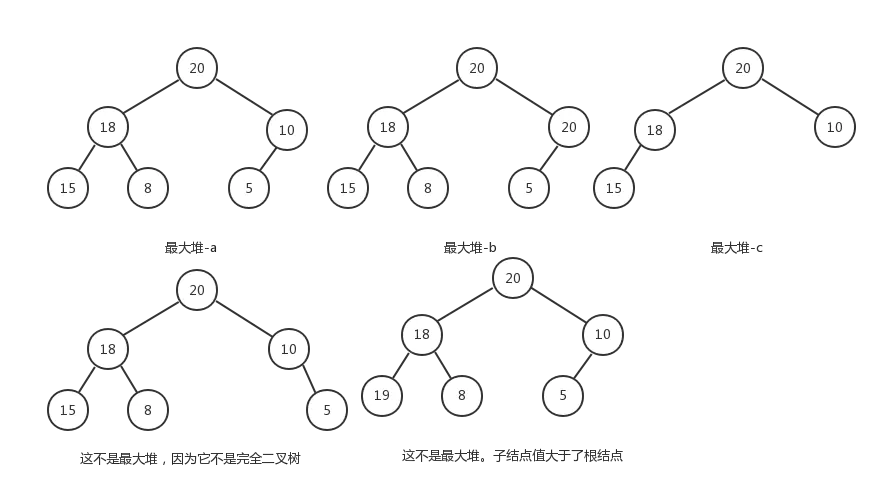
\includegraphics[width=0.7\textwidth]{最大堆.png}
    \caption{最大堆的示意图} % 图片标题
    \label{fig:最大堆} % 图片标签，用于引用
\end{figure}

\begin{figure}[H]
    \centering
    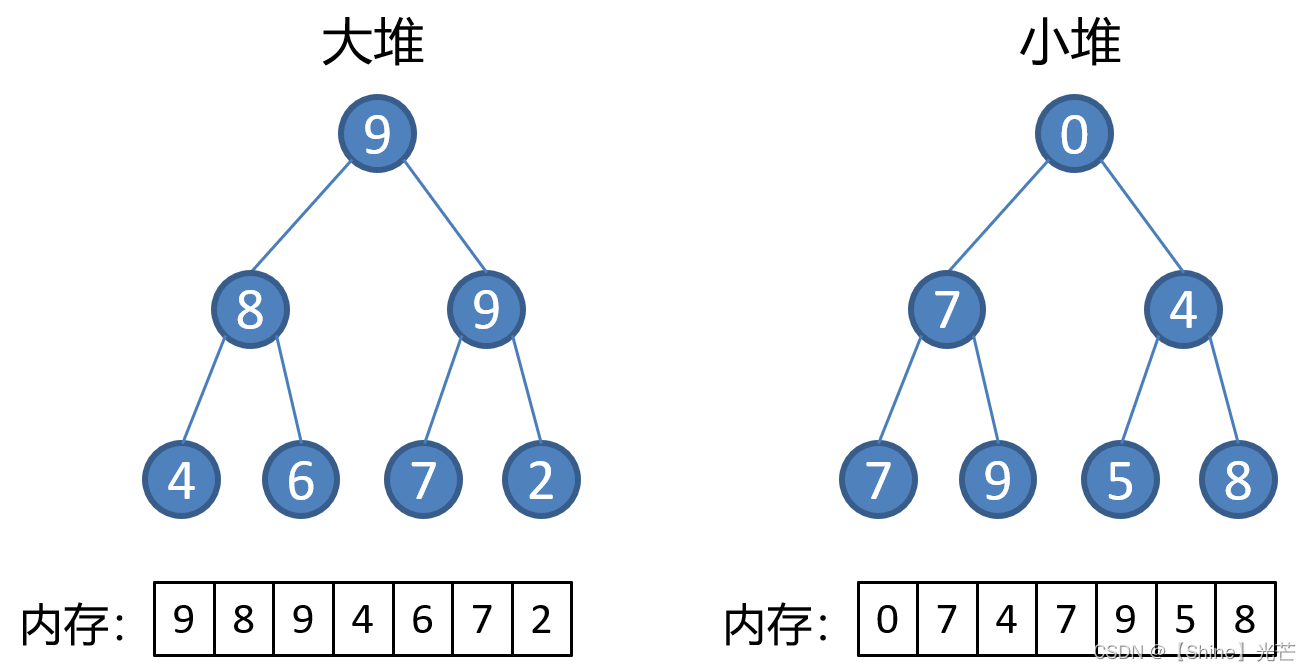
\includegraphics[width=0.7\textwidth]{堆1.png}
    \caption{最大堆和最小堆} % 图片标题
    \label{fig:最大堆和最小堆} % 图片标签，用于引用
\end{figure}

上一小节介绍的优先队列正是基于堆实现的：它通过为每个任务的重要程度编号，把编号大的任务放在堆顶，
从而快速取出最重要的任务；堆的调整算法很快，因此优先队列被广泛应用于\textbf{任务管理}中。
优先队列的容器用法已在上一小节给出，这里不再重复。

\subsubsection{映射}

映射是一种关联容器，它是一个\textbf{键值对}的集合，其中每个键都是唯一的，值可以重复。
映射有两种主流实现：基于哈希表的实现查找、插入、删除的平均时间复杂度是$O(1)$；
基于红黑树的实现则是$O(logN)$，但能保持键有序。

\textbf{红黑树（Red-Black Tree）}是一种随机查找速度比较快的\textbf{平衡二叉树}\footnote{
    平衡二叉树，也叫AVL树，它或者是一棵空树，或者具有以下性质的二叉排序树：它的左子树和右子树的高度之差（平衡因子）的绝对值不超过1，且它的左子树和右子树都是一棵平衡二叉树}
，它的查找、插入、删除操作的时间复杂度都是$O(logN)$\footnote{
    O(logN)表示时间复杂度，N是问题的规模，O表示运行消耗时间的上界
}。

\textbf{哈希表（HashTable）}是一种\textbf{散列表}，它通过\textbf{哈希函数}将键映射到值。
由于其使用计算来查找，因此，查找操作的平均时间复杂度是$O(1)$
\footnote{常数的时间复杂度意味着不管问题的规模如何，
对于同一个长度的HashTable，算法的运行时间都不会随着问题的规模增加而增长。}。
但是哈希表的建立比较困难，需要消耗很多资源。
而且存储长度有限，当元素过多时，哈希表的性能会下降。当哈希表满时，需要执行\textbf{再散列（Rehashing）}，解决\textbf{哈希冲突（Hash Collision）}问题，
这个过程需要消耗大量时间。

两者各有优劣，在实际应用中，需要根据具体问题选择。
红黑树型映射的STL容器是$map$，哈希表型映射的STL容器是$unordered\_map$。

\begin{example}
\texttt{map} 与 \texttt{unordered\_map} 的基本用法：
\begin{tcode}
#include <iostream>
#include <map>
#include <unordered_map>
#include <string>

int main() {
    std::map<std::string,int> score;            //红黑树实现，按键有序
    score["alice"] = 90;                        //插入或修改
    score.emplace("bob", 85);
    std::cout << score["alice"] << std::endl;   //按键访问
    std::cout << score.count("carol") << std::endl; //判断键是否存在：0
    for(auto& [name, s] : score){               //遍历，按字母序输出
        std::cout << name << ": " << s << std::endl;
    }

    std::unordered_map<std::string,int> fastScore; //哈希表实现，无序但更快
    fastScore["alice"] = 90;
    return 0;
}
\end{tcode}
\end{example}

\begin{note}
具体用法请自行查阅相关文档：

\url{https://zh.cppreference.com/w/cpp/container/map}

注意：\texttt{map} 的 \texttt{operator[]} 在键不存在时会\textbf{自动插入}一个默认值，
只想查询不想改动时，请用 \texttt{find()} 或 \texttt{count()}。
\end{note}

\begin{exercise}
使用 \texttt{std::map<std::string,int>} 统计一段文字中每个单词出现的次数，并按键的字母序打印结果。
\end{exercise}

\subsubsection{迭代器与失效}

迭代器是一种检查容器内元素并遍历元素的数据类型，通常用于对C++中各种容器内元素的访问，
但不同的容器有不同的迭代器，初学者可以将迭代器理解为一个可以\textbf{自动向后移动的指针}。

常用的可迭代的容器有：

\begin{enumerate}
    \item 序列容器：$array$、$vector$、$deque$、$list$、$forward\_list$等
    \item 关联容器：$set$、$map$、$multimap$等
\end{enumerate}

$queue$、$stack$、$priority\_queue$是容器适配器，必须满足一定规则，没有迭代器。

对于可迭代容器，一般可以使用.begin()和.end()方法获取迭代器，.begin()方法返回指向第一个元素的迭代器，
.end()方法返回指向最\textbf{后一个元素的迭代器的下一位置}。

\begin{example}
用迭代器遍历容器：
\begin{tcode}
#include <iostream>
#include <vector>

int main() {
    std::vector<int> vec{1,2,3,4,5,6,7,8,9,0};
    for(auto it = vec.begin();it != vec.end();++it){
        std::cout << *it << std::endl;
    }
    return 0;
}
\end{tcode}
\end{example}

也可以简写为范围for循环：

\begin{tcode}
for (auto it : vec) {
    std::cout << it << std::endl;
}
\end{tcode}

\begin{example}
迭代器的常见修改操作：
\begin{tcode}
#include <algorithm> //sort、remove_if、iter_swap 都在这个头文件里

std::vector<int> vec{1, 2, 3, 4, 5, 6, 7, 8, 9, 0};
vec.erase(vec.begin()+5);            //删除第6个元素
vec.erase(vec.begin()+5, vec.end()); //删除第6个元素之后的所有

std::vector<int> vec1{1, 2, 3, 4, 5, 6, 7, 8, 9, 0};
std::iter_swap(vec1.begin(), vec1.begin()+1); //交换第一个和第二个元素

std::vector<int> vec2{1, 2, 3, 4, 5, 6, 7, 8, 9, 0};
std::sort(vec2.begin(), vec2.end(), [](int a, int b){
    return a >= b;                  //降序排序
});

//remove_if 只把不满足条件的元素挪到前面，并不真正删除
//正确姿势是 erase-remove 惯用法：
vec2.erase(std::remove_if(vec2.begin(), vec2.end(), [](int a){
    return a > 5;
}), vec2.end());                    //这才真正删除了大于5的元素
\end{tcode}
\end{example}

\begin{note}
\texttt{std::remove\_if} 并不会改变容器大小，它只是把"要保留"的元素搬到前面、返回新的逻辑结尾迭代器，
必须配合 \texttt{erase} 才能完成删除——这就是著名的 erase-remove 惯用法。忘记接 \texttt{erase}，
容器里会留下一堆"僵尸元素"。更多迭代器内容见 cppreference：

\url{https://zh.cppreference.com/w/cpp/iterator}
\end{note}

\textbf{迭代器失效。}

迭代器失效指的是迭代器因为某些操作而不再指向原来的元素，
或者不再保持有效的状态，这样的迭代器如果继续使用，可能会导致未定义行为，包括程序崩溃。
通俗的理解就是，当你对容器进行了操作时，更改了容器的大小，但是迭代器仍然指向原来的位置，
这样就会导致读取错误的内存，这就是迭代器失效。

\begin{tcode}
std::vector<int> vec={1,2,3,4,5,6,7,8,9,10};
for(auto it = vec.begin(); it != vec.end(); ++it){
    if(*it % 2 == 0){
        vec.erase(it); //错误示范：erase之后it已经失效
    }
}
\end{tcode}

看上面的代码，当执行到vec.erase(it)时，it已经失效，因为执行了erase之后，
vec的大小发生了变化，这导致了迭代器失效。

在实践过程中，下面的几种情况下迭代器会失效，需要\textbf{避免}出现：
\begin{enumerate}
    \item 当执行erase方法时，指向删除节点的迭代器失效，指向删除节点之后的迭代器也全部失效
    \item 当进行push\_back()方法时，end操作返回的迭代器肯定失效
    \item 当插入（push\_back）一个元素后，capacity返回值与插入之前相比有改变，
    则说明容器整体搬了家，此时所有迭代器都会失效
    \item 当插入（push\_back）一个元素后，如果空间未重新分配，指向插入位置之前的元素的迭代器仍然有效，但指向插入位置之后元素的迭代器全部失效
\end{enumerate}

对于关联容器，删除一个键值对只会使当前这个迭代器失效，别的迭代器不会受到影响，
这可能是由于底层使用红黑树实现的原因。但是实际应用中，仍然不应该冒这个风险，因此，
必须\textbf{坚决避免迭代器失效问题的发生}。

在具体的应用中，我们在使用迭代器遍历时，应该注意不要对容器进行增删操作，更不应该改变容器的大小。
正确的删除写法是利用 erase 的返回值——它会返回指向被删元素\textbf{下一个}元素的有效迭代器：

\begin{example}
遍历中安全删除元素：
\begin{tcode}
std::vector<int> vec={1,2,3,4,5,6,7,8,9,10};
for(auto it = vec.begin(); it != vec.end(); ){ //注意：这里没有++it
    if(*it % 2 == 0){
        it = vec.erase(it); //erase返回下一个有效迭代器
    }else{
        ++it;
    }
}
\end{tcode}
\end{example}

\begin{conclusion}
迭代器失效自救指南：

\begin{itemize}
\item 遍历容器时不要随手增删元素，先想清楚迭代器下一步指向哪；
\item 删除元素用 \texttt{it = vec.erase(it);} 接住返回值，而不是 \texttt{vec.erase(it);} 后继续用旧迭代器；
\item push\_back 导致扩容后，之前保存的所有迭代器、指针、引用全部作废，需要遍历就重新获取；
\item 批量按条件删除，优先考虑 erase-remove 惯用法，一行解决，不容易写错。
\end{itemize}
\end{conclusion}

\begin{exercise}
把"错误示范"的代码抄下来运行，观察运行结果或崩溃现象；再用"遍历中安全删除元素"的写法修复它，
删除所有偶数并打印剩余的奇数。
\end{exercise}
